\chapter{IS Audit}
\label{audit}

Audit viene dal latino \textit{audere}, ovvero ascoltare.

Indagine forense, cerca recuperare informazioni dai sistemi informatici, ora è
difficile per via del cloud.

\paragraph*{Definizione}

Un processo sistematico nel quale un team qualificato, competente e
indipendente ottiene in maniera obiettiva prove\footnote{La evidence significa
prova e tutte le evidenze del tipo ``ho sentito che'' non sono prove, e per
questo non possono far parte dell'audit.} e valutano le asserzioni riguardo ai
processi con l'obiettivo di creare un'opinione a riguardo e riportare il grado
in cui l'asserzione è implementata.


\section{Qualità di un Auditor}

L'auditor deve avere le seguenti qualifiche:
\begin{itemize}
\item Indipendenza professionale: gli auditor agiscono indipendentemente dal
gruppo che subisce l'audit;
\item Indipendenza organizzativa: l'auditor non deve avere interessi o
dipendenze gerarchiche con l'unità aziendale sotto audit. L'auditor sta sotto
il diretto controllo del CEO.
\end{itemize}

L'auditor è in un processo di formazione continua. Per esempio le
certificazioni richiedono continui aggiornamenti dal punto di vista
professionale.

\section{IS Audit Definition}

Un IS audit può essere definito come una qualsiasi \textbf{revisione} che 
valuta in tutto o in parte un sistema automatizzato di elaborazione delle 
informazioni, dei relativi processi non automatizzati e le relative interfacce.

La prima attività che fa l'auditor è guadagnare la comprensione del soggetto
che sta analizzando (es. contesto aziendale).
La seconda è valutare i controlli e l'ultima è testare i controlli, come
mostrato nella Figura \ref{fig:is:audit:definition}.

Cerca di capire il contesto aziendale, dove sta accendo e le relazioni tra le
unità aziendali e cerca di prendere contatto con la realtà aziendale che lo
circonda.


\begin{figure}[h!]
	\begin{center}
		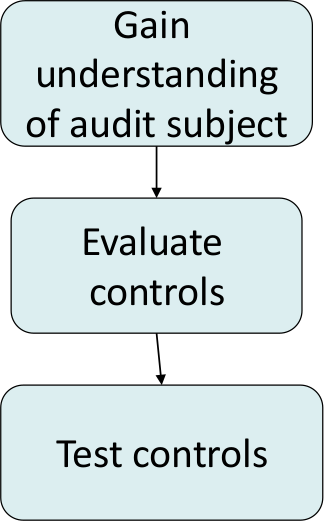
\includegraphics[scale=0.3]{res/img/is_audit_definition.png}
	\end{center}
	\caption{Diagramma di flusso (semplificato) per il processo di IS
audit.}
	\label{fig:is:audit:definition}
\end{figure}

\section{Pianificazione dell'audit}

Attualmente la pianificazione dell'audit viene fatta ogni 3 anni.
Esistono due tipologie di Audit:
\begin{enumerate}
\item Breve termine: su cosa c'è bisogno di fare audit quest'anno?
\item Lungo termine: su cosa dobbiamo pianificare di fare audit nel futuro?
\end{enumerate}

Durante un audit è importante porsi delle domande per poter portare
correttamente a termine il lavoro. Che cosa dobbiamo testare per primo?
Per poter rispondere a questo quesito dobbiamo considerare le seguenti
domande:

\begin{itemize}
\item Qual è la parte del nostro business più sensibile al rischio?
\item Che sistemi di business/IS stanno cambiando?
\item Ci sono nuovi tool di valutazione?
\item Che regole dobbiamo testare?
\item Ci sono nuove regole da testare?
\end{itemize}

L'audit è molto importante soprattutto in zone definite come critiche. Zone di
guerra sono spesso soggette a corruzione, e quindi il lavoro di audit risulta
essere difficile da eseguire.

\section{Procedura estesa di audit}

Come già detto, è importante capire la realtà in cui ci si trova. È poi
fondamentale eseguire un \textit{risk assessment} per capire le zone di rischio
maggiore.
Infine viene preparato il piano, in cui verranno controllate diverse aree.
Vengono esaminati anche lavori precedenti, con la revisione della
documentazione
e vengono eseguite interviste. Le interviste sono molto importanti perché
permettono, con le giuste domande, di acquisire molte informazioni.
I \textit{test di compliance} eseguono i controlli sulla corretta esecuzione
dei
test.

Viene poi steso il rapporto di audit, a cui a seguire ci sono delle attività
secondarie. Queste attività secondarie dipendono da che tipo di audit è:
\begin{itemize}
\item Esterno: queste attività di solito non vengonono eseguite;
\item Interno: queste attività vengono continuate.
\end{itemize}

La consegna dell'Audit implica una interazione con chi non gestisce
correttamente un determinato processo: è infatti importante non solamente
consegnare l'Audit ma anche discutere dei problemi presenti per poter
migliorare
la situazione.

\subsection{Step 1: Ottenere la comprensione dell'area soggetta ad audit}

Questa è la fase iniziale, che comprende diversi passi che devono essere
eseguiti sistematicamente.
Questi passi sono:
\begin{itemize}
\item Tour delle strutture relative all'audit;
\item Lettura dei documenti (es. risk assessment, documenti di processi andati
male);
\item Revisione del piano di business e del piano IT strategico:
\item Interviste alle persone chiave per capire il business dell'azienda;
\item Lettura degli audit precedenti;
\item Capire qual è la regolamentazione da applicare;
\item Identificare le aree che sono state esternalizzate.
\end{itemize}

\subsection[Step 2: Risk assessment e Piano di Audit]{Step 2: Risk
assessment e Piano di Audit\protect\footnote{Chiesti all'esame dal
prof.}}

\subsubsection{Effettuare il risk assessment}

\paragraph*{Rischio inerente}

È il rischio legato all'attività che viene svolta\footnote{Legato al business.}
(es. per una fabbrica di fuochi di artificio il rischio inerente è
l'esplosione).

Per esempio, per una farmacia, il rischio inerente è:
\begin{itemize}
\item Truffa;
\item Rapina.
\end{itemize}

\paragraph*{Rischio di controllo}

Un rischio che non può essere rilevato da un controllo interno. Ovvero un
rischio che possa passare inosservato (es. per una banca: l'accesso di un ladro
all'account di qualcun altro che però non viene rilevato).


\paragraph*{Rischio del rilevamento}

Un auditor non riesce a rilevare un problema che esiste (es. nel caso
di una banca avviene una frode che non viene rilevata).

\paragraph*{Rischio generale dell'Audit}

Combinazione dei rischi precedenti.


\subsubsection{Preparare un piano di Audit}

È importante prevedere un lavoro di Audit che sia pianificabile in tempo:
prendere un lavoro che deve essere svolto in pochissimo tempo non è
fruttuoso, in quanto viene eseguito solitamente male e si ha di
ritorno una cattiva pubblicità. In questo segmento di mercato, per farsi una
buona reputazione ci si mette tanto tempo; mentre per rovinarsela ci vuole
pochissimo.
Quindi se si vede che non c'è abbastanza tempo per eseguire quel determinato
lavoro è meglio non accettarlo.
È importante avere anche i giusti spazi: la disponibilità delle segreterie per
eseguire fotocopie di documenti per esempio\footnote{Solitamente, questa cosa
vale in base al NDA firmato.} migliora di sicuro la qualità del lavoro svolto
(questo vale anche, per esempio, per avere un piccolo spazio/ufficio su cui
eseguire l'audit). Per i documenti non cartacei, come quelli elettronici,
devono essere rilasciate garanzie su dove vengono salvati, come ad esempio se è
presente la cifratura sul dispositivo di storicizzazione o meno.

L'audit si sviluppa su un approccio basato sul rischio e vengono inclusi
obiettivi, scopo, tempo e risorse richieste per l'audit.

La pianificazione dev'essere eseguita correttamente, in quanto solitamente il
tempo per eseguire un audit non è molto e sono presenti \textit{deadline}
strette.

\paragraph{Vocabolario della Pianificazione dell'Audit}

In una pianificazione dell'audit, è importante tenere a mente i seguenti
vocaboli:
\begin{itemize}
\item \textbf{Soggetto dell'audit:} l'area che viene auditata;
\item \textbf{Obiettivo dell'audit:} lo scopo dell'audit (es. determinare se un
processo è controllato bene);
\item \textbf{Contesto dell'audit:} limitare l'audit ad uno specifico sistema,
funzione, oggetto.
\end{itemize}


\paragraph*{Esempio}
Un esempio per prendere confidenza con la terminologia del piano
di audit è riportato nella Figura~\ref{fig:audit:plan:vocabulary:example}.

\begin{figure}[H]
	\begin{center}
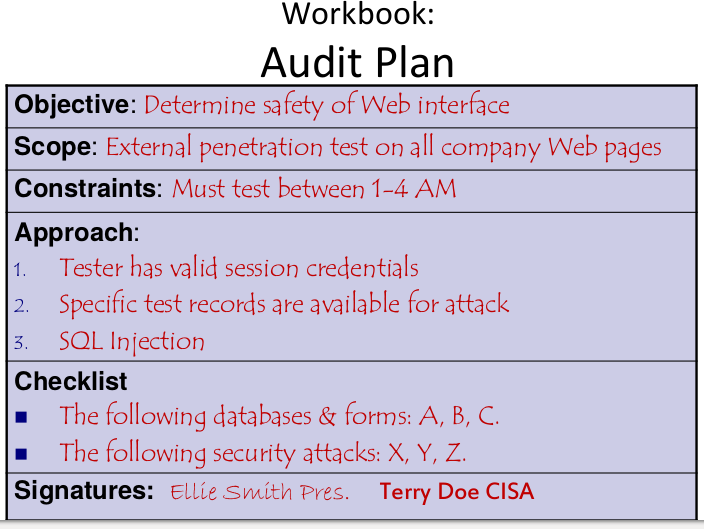
\includegraphics[scale=0.3]{res/img/audit_plan_vocabulary_example.png}
	\end{center}
	\caption{Esempio per prendere confidenza con i termini dell'audit plan.}
	\label{fig:audit:plan:vocabulary:example}
\end{figure}

\subsection{Step 3: Aggiungere dettagli al piano}

Gli step sono: (i) tradurre gli oggetti dell'audit in oggetti più specifici,
(ii) identificare e selezionare l'approccio di audit per testare e verificare i
controlli, (iii) identificare gli individui da intervistare, (iv) ottenere le
policy, standard, procedure e linee guida aziendali e (v) sviluppare degli
strumenti e delle metodologie di audit.

\subsection{Step 4: Valutare l'area di audit}

Vengono usati \textit{strumenti} di tipo generale e osservazioni sul campo.
Queste osservazioni sul campo sono sempre molto utili, perché permettono di
vedere effettivamente come i dipendenti stanno lavorando (es. osservando
un amministratore di sistema si potrebbe scoprire se è stata applicata una
corretta \textit{segregation of duties}) e permette di scoprire elevate
criticità.

\subsection{Step 5: Valutare i controlli}

È sempre molto importante lavorare sulla struttura organizzativa, che deve
essere aggiornata in maniera continua.
Altri punti importanti:
\begin{itemize}
\item \textbf{Revisione dell'organizzazione IS:} separation of duties;
\item \textbf{Revisione delle policy, standard, procedure di IS:} definite,
aggiornate periodicamente. Sulle policy viene indicato il versionamento del
documento (versione, data, firma di chi ha autorizzato);
\item \textbf{Revisione della documentazione IS};
\item \textbf{Intervista del personale:} segregation of duties, security
awareness, competenze relative al proprio lavoro. È importante conoscere come i
dipendenti lavorano all'interno dell'azienda, senza porre domande troppo
sospette. Una domanda molto importante da fare è: \textit{"come si trova sul
lavoro?"} in quanto quando ci si trova ad eseguire dei \textit{task}
per cui non si è adatti ci sono molto probabilmente delle difficoltà. Questo da
il \textit{sentiment} della situazione aziendale;
\item \textbf{Osservare il personale:} documentare tutto con un livello
sufficiente di dettaglio, questa documentazione deve essere tale
da fornire evidenza dei fatti.
\end{itemize}


\subsubsection{Tipologie di controlli}

I controlli sono principalmente di tre tipi:

\begin{itemize}
\item \textbf{Controlli correttivi}: controlli che risolvono i problemi e
evitano che quella tipologia di problema risorga nel futuro. Ad esempio il
\textit{contingency plan}\footnote{Il contingency plan è quella
attività che permette l'erogazione di un servizio anche ad un livello
degradato.} è uno di questi.

\item \textbf{Controlli detettivi}: controllano l'integrità delle
informazioni, (es. l'integrità dei database). Esistono software
molto costosi che permettono di analizzare i log di sistema, per carpire
maggiori informazioni.

\item \textbf{Controlli preventivi}: i controlli più difficili da eseguire, ma
quelli che permettono di far risparmiare di più, poichè permettono di evitare
il rischio. Alcune cose che solitamente sono da verificare è che i dischi siano
criptati e che il personale sia adeguatamente aggiornato e preparato.
Il personale è fondamentale: persone che non sono adatte al ruolo faranno male
il lavoro e verranno (o si faranno) licenziare subito, causando un
elevato \textit{turnover}. Questo indice deve essere basso per un'azienda e
costituisce un problema enorme in quanto prendere una persona costa risorse, in
tempo e soldi. La soglia di \textit{turnover} non deve mai superare il 5-7\%.
\end{itemize}

\begin{figure}[H]
	\begin{center}
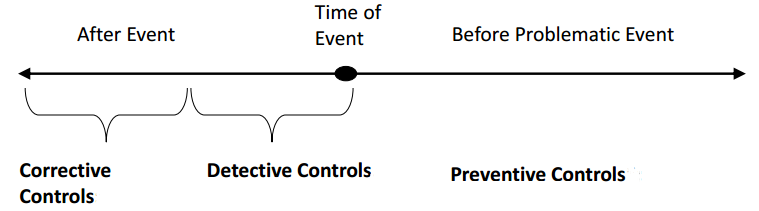
\includegraphics[scale=0.4]{control_timeline}
	\end{center}
	\caption{Linea del tempo dei vari tipi di controllo.}
\end{figure}


\subsubsection{Manutenzione dei controlli}

Questi tipi di controlli sono di natura qualitativa.

\textbf{Controlli in overlap:} va a compensare il rischio di controllo, in modo
che se un controllo non trova il problema possa trovarlo un altro.

\textbf{Controllo compensativo:} supporta un controllo più debole.

\subsection{Step 6 e 7: Test dell'audit}

\begin{itemize}
\item \textbf{Evidence:} i risultati (\emph{findings}) sono basati su prove e
fatti sufficienti e affidabili e su una corretta interpretazione dell'evidenza;

\item \textbf{Documentazione:} il lavoro di audit e l'evidenza
devono essere completamente documentate per supportare le conclusioni;

\item \textbf{Supervisione:} lo staff di audit viene supervisionato per
assicurare che l'audit venga eseguito in modo professionale;

\item \textbf{Scetticismo professionale:} bisogna essere scettici nei confronti
dei controlli in modo da verificare tutto quello che deve essere verificato.
Quando si incontrano irregolarità bisogna andare in profondità, riportandole
in maniera corretta. Anche le controparti vanno informate e questa tipologia di
azioni non va mai eseguita di ``nascosto''. Lo stesso discorso va fatto anche
se la controparte è in malafede. In caso venga scoperta una controparte che è in
malafede bisogna avvisare immediatamente riguardo alla situazione, perché è
presente il rischio che la controparte cancelli le prove che la colpevolizzano.
\end{itemize}






\subsubsection{Step 6: Test di conformità}
I test di conformità rispondono alla domanda \textit{
``i controlli sono presenti e eseguiti in maniera consistente?''}.

\paragraph*{Esempio di Controllo:} il software in produzione è controllato?
\begin{itemize}
\item \textbf{Test:} I file eseguibili vengono buildati dal codice sorgente che
sta nel repository? Se questo non accade è un grave problema, perché significa
che si sta usando del software in produzione che è diverso da quello che è
presente nel repository;
\item \textbf{Test:} Sono state seguite le procedure adeguate durante la
release? Nelle aziende grosse, è presente un libro dei test, in cui chi è
responsabile appone una firma prima di rilasciare una certa versione del
software.
\end{itemize}


\subsubsection{Step 7: Test sostanziali}
I test sostanziali verificano che tutto funzioni come dovrebbe.
Se i risultati dei test di conformità sono scarsi, mi aspetto che i controlli
sostanziali siano più numerosi in tipo e numero.

\paragraph*{Esempio di Audit:} la sezione finanziaria sulle vendite è accurata?

\begin{itemize}
\item \textbf{Test:} tracciare il processing di un esempio di transazione
attraverso il sistema, eseguendo i calcoli manualmente;
\item \textbf{Test:} testare le condizioni di errore.
\end{itemize}


\subsubsection{Campionamento}
Si ricorre al campionamento quando considerazioni di tempo e costi
precludono una verifica di \emph{tutti} gli eventi e
\emph{tutte} le transazioni di una popolazione predefinita.
La \textbf{popolazione} consiste di un intero gruppo di oggetti
che devono essere esaminati.
Il sottoinsieme della popolazione usato per
eseguire il testing è chiamato \textbf{campione}. Il campionamento
è utilizzato per inferire caratteristiche riguardo alla popolazione,
basandosi sul campione.

Esistono due approcci generali per il campionamento dell'audit:
\paragraph*{Campionamento statistico:} ci sono tecniche standard, fornisce un
\textit{intervallo di confidenza}\footnote{L'\textbf{intervallo
di confidenza} è la probabilità che le caratteristiche del
campione siano vere rappresentazioni delle caratteristiche della
popolazione. Questo coefficiente viene rappresentato con un $\epsilon$,
il quale più piccolo è e meglio è. Solitamente, si usa un intervallo di
confidenza del 90\%.}. Se abbiamo N item, con un campione di
$\sqrt{N}$ elementi garantisce una precisione del 99.9\%.
$$
(1 - 1/100)^K
$$
\paragraph*{Campionamento non stastistico:} si basa sul giudizio
dell'auditor e soprattutto su informazioni di contorno, come per
esempio quali item/transactions sono/comportano il maggior rischio?
Con questo approccio si perde la rappresentatività
del campione statistico, ma si trovano delle evidenze su ciò che
si sta realmente cercando.
